

\tikzset{every picture/.style={line width=0.75pt}} %set default line width to 0.75pt        

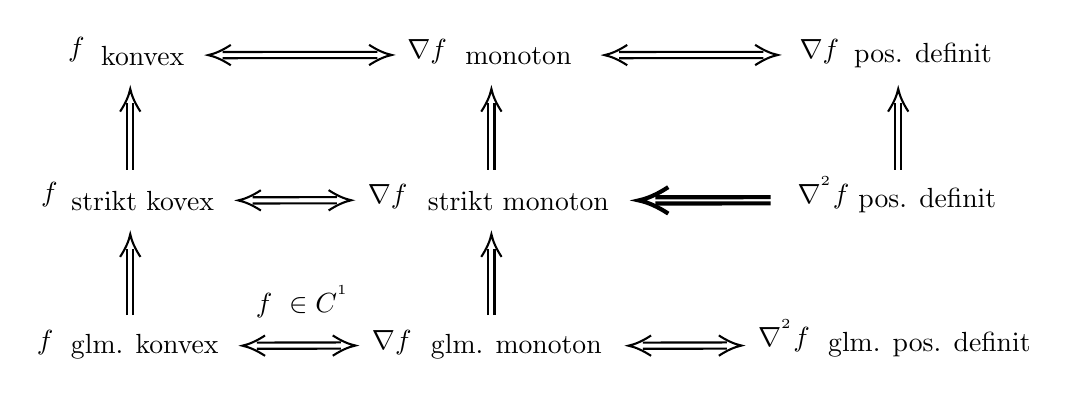
\begin{tikzpicture}[x=0.75pt,y=0.75pt,yscale=-1,xscale=1]
%uncomment if require: \path (0,184.43749237060547); %set diagram left start at 0, and has height of 184.43749237060547




%Straight Lines [id:da6931552921369328] 
\draw [line width=0.75]    (502.5,79.01) -- (502.5,47.01)(505.5,79.01) -- (505.5,47.01) ;
\draw [shift={(504,40.01)}, rotate = 450] [color={rgb, 255:red, 0; green, 0; blue, 0 }  ][line width=0.75]    (10.93,-4.9) .. controls (6.95,-2.3) and (3.31,-0.67) .. (0,0) .. controls (3.31,0.67) and (6.95,2.3) .. (10.93,4.9)   ;




%Straight Lines [id:da5376916843087101] 
\draw [line width=0.75]    (306.5,79.01) -- (306.5,47.01)(309.5,79.01) -- (309.5,47.01) ;
\draw [shift={(308,40.01)}, rotate = 450] [color={rgb, 255:red, 0; green, 0; blue, 0 }  ][line width=0.75]    (10.93,-4.9) .. controls (6.95,-2.3) and (3.31,-0.67) .. (0,0) .. controls (3.31,0.67) and (6.95,2.3) .. (10.93,4.9)   ;

%Straight Lines [id:da9601126151289101] 
\draw [line width=0.75]    (306.5,149.01) -- (306.5,117.01)(309.5,149.01) -- (309.5,117.01) ;
\draw [shift={(308,110.01)}, rotate = 450] [color={rgb, 255:red, 0; green, 0; blue, 0 }  ][line width=0.75]    (10.93,-4.9) .. controls (6.95,-2.3) and (3.31,-0.67) .. (0,0) .. controls (3.31,0.67) and (6.95,2.3) .. (10.93,4.9)   ;





%Straight Lines [id:da17111805237135647] 
\draw [line width=0.75]    (132.5,79.01) -- (132.5,47.01)(135.5,79.01) -- (135.5,47.01) ;
\draw [shift={(134,40.01)}, rotate = 450] [color={rgb, 255:red, 0; green, 0; blue, 0 }  ][line width=0.75]    (10.93,-4.9) .. controls (6.95,-2.3) and (3.31,-0.67) .. (0,0) .. controls (3.31,0.67) and (6.95,2.3) .. (10.93,4.9)   ;

%Straight Lines [id:da6402722120192785] 
\draw [line width=0.75]    (132.5,149.01) -- (132.5,117.01)(135.5,149.01) -- (135.5,117.01) ;
\draw [shift={(134,110.01)}, rotate = 450] [color={rgb, 255:red, 0; green, 0; blue, 0 }  ][line width=0.75]    (10.93,-4.9) .. controls (6.95,-2.3) and (3.31,-0.67) .. (0,0) .. controls (3.31,0.67) and (6.95,2.3) .. (10.93,4.9)   ;


%Straight Lines [id:da19646642044249396] 
\draw [line width=1.5]    (442.5,95.15) -- (387,95.21)(442.5,92.15) -- (387,92.21) ;
\draw [shift={(379,93.72)}, rotate = 359.93] [color={rgb, 255:red, 0; green, 0; blue, 0 }  ][line width=1.5]    (14.21,-6.37) .. controls (9.04,-2.99) and (4.3,-0.87) .. (0,0) .. controls (4.3,0.87) and (9.04,2.99) .. (14.21,6.37)   ;

%Straight Lines [id:da012310767209407603] 
\draw [line width=0.75]    (439,25.15) -- (369.5,25.22)(439,22.15) -- (369.5,22.22) ;
\draw [shift={(362.5,23.72)}, rotate = 359.95] [color={rgb, 255:red, 0; green, 0; blue, 0 }  ][line width=0.75]    (10.93,-4.9) .. controls (6.95,-2.3) and (3.31,-0.67) .. (0,0) .. controls (3.31,0.67) and (6.95,2.3) .. (10.93,4.9)   ;
\draw [shift={(446,23.65)}, rotate = 179.95] [color={rgb, 255:red, 0; green, 0; blue, 0 }  ][line width=0.75]    (10.93,-4.9) .. controls (6.95,-2.3) and (3.31,-0.67) .. (0,0) .. controls (3.31,0.67) and (6.95,2.3) .. (10.93,4.9)   ;
%Straight Lines [id:da8068390743979135] 
\draw [line width=0.75]    (421.5,165.16) -- (381,165.21)(421.5,162.16) -- (381,162.21) ;
\draw [shift={(374,163.72)}, rotate = 359.91999999999996] [color={rgb, 255:red, 0; green, 0; blue, 0 }  ][line width=0.75]    (10.93,-4.9) .. controls (6.95,-2.3) and (3.31,-0.67) .. (0,0) .. controls (3.31,0.67) and (6.95,2.3) .. (10.93,4.9)   ;
\draw [shift={(428.5,163.65)}, rotate = 179.92] [color={rgb, 255:red, 0; green, 0; blue, 0 }  ][line width=0.75]    (10.93,-4.9) .. controls (6.95,-2.3) and (3.31,-0.67) .. (0,0) .. controls (3.31,0.67) and (6.95,2.3) .. (10.93,4.9)   ;
%Straight Lines [id:da7137872354673338] 
\draw [line width=0.75]    (235.5,165.16) -- (195,165.21)(235.5,162.16) -- (195,162.21) ;
\draw [shift={(188,163.72)}, rotate = 359.91999999999996] [color={rgb, 255:red, 0; green, 0; blue, 0 }  ][line width=0.75]    (10.93,-4.9) .. controls (6.95,-2.3) and (3.31,-0.67) .. (0,0) .. controls (3.31,0.67) and (6.95,2.3) .. (10.93,4.9)   ;
\draw [shift={(242.5,163.65)}, rotate = 179.92] [color={rgb, 255:red, 0; green, 0; blue, 0 }  ][line width=0.75]    (10.93,-4.9) .. controls (6.95,-2.3) and (3.31,-0.67) .. (0,0) .. controls (3.31,0.67) and (6.95,2.3) .. (10.93,4.9)   ;
%Straight Lines [id:da3667450709373552] 
\draw [line width=0.75]    (233.5,95.16) -- (193,95.21)(233.5,92.16) -- (193,92.21) ;
\draw [shift={(186,93.72)}, rotate = 359.91999999999996] [color={rgb, 255:red, 0; green, 0; blue, 0 }  ][line width=0.75]    (10.93,-4.9) .. controls (6.95,-2.3) and (3.31,-0.67) .. (0,0) .. controls (3.31,0.67) and (6.95,2.3) .. (10.93,4.9)   ;
\draw [shift={(240.5,93.65)}, rotate = 179.92] [color={rgb, 255:red, 0; green, 0; blue, 0 }  ][line width=0.75]    (10.93,-4.9) .. controls (6.95,-2.3) and (3.31,-0.67) .. (0,0) .. controls (3.31,0.67) and (6.95,2.3) .. (10.93,4.9)   ;
%Straight Lines [id:da16014383432778323] 
\draw [line width=0.75]    (253,25.15) -- (178.5,25.22)(253,22.15) -- (178.5,22.22) ;
\draw [shift={(171.5,23.72)}, rotate = 359.95] [color={rgb, 255:red, 0; green, 0; blue, 0 }  ][line width=0.75]    (10.93,-4.9) .. controls (6.95,-2.3) and (3.31,-0.67) .. (0,0) .. controls (3.31,0.67) and (6.95,2.3) .. (10.93,4.9)   ;
\draw [shift={(260,23.65)}, rotate = 179.95] [color={rgb, 255:red, 0; green, 0; blue, 0 }  ][line width=0.75]    (10.93,-4.9) .. controls (6.95,-2.3) and (3.31,-0.67) .. (0,0) .. controls (3.31,0.67) and (6.95,2.3) .. (10.93,4.9)   ;


% Text Node
\draw (108,20.87) node   {$f$};
% Text Node
\draw (140,23.87) node  [align=left] {konvex};
% Text Node
\draw (277,22) node   {$\nabla f$};
% Text Node
\draw (321,24) node  [align=left] {monoton};
% Text Node
\draw (466,22) node   {$\nabla f$};
% Text Node
\draw (516,24) node  [align=left] {pos. definit};
% Text Node
\draw (95,91) node   {$f$};
% Text Node
\draw (140,94) node  [align=left] {strikt kovex};
% Text Node
\draw (258,92) node   {$\nabla f$};
% Text Node
\draw (321,94) node  [align=left] {strikt monoton};
% Text Node
\draw (468,90) node   {$\nabla ^{^{2}} f$};
% Text Node
\draw (518,94) node  [align=left] {pos. definit};
% Text Node
\draw (93,162) node   {$f$};
% Text Node
\draw (141,164) node  [align=left] {glm. konvex};
% Text Node
\draw (260,162) node   {$\nabla f$};
% Text Node
\draw (320,164) node  [align=left] {glm. monoton};
% Text Node
\draw (449,159) node   {$\nabla ^{^{2}} f$};
% Text Node
\draw (519,163) node  [align=left] {glm. pos. definit};
% Text Node
\draw (217,142.44) node   {$f\ \in C^{^{1}}$};


\end{tikzpicture}
